

\documentclass[10pt]{beamer}

\linespread{1.0}

\usetheme{Pittsburgh}
%\usetheme {CambridgeUS}%{Goettingen}%{Berkeley}%{Montpellier}%{Antibes}%{Dresden}%{Madrid}%{Dresden}%{Darmstadt}%{Warsaw}%{Pittsburgh}
\usefonttheme{serif}%{structurebold}%{structuresmallcapsserif}%{professionalfonts}
\usepackage[english]{babel}
%\usepackage[latin1]{inputenc}
\usepackage{hyperref}
%\usecolortheme{beaver}
%\usecolortheme{crane}

\setbeamercovered{transparent}


\usepackage{latexsym}
\usepackage{amsmath}
\usepackage{times}
\usepackage{MinionPro}
\usepackage{hyperref}
\usepackage{tikz}
\usepackage{verbatim}
\usepackage{natbib}
\usepackage{color, colortbl}
\usepackage{appendix}
\usepackage{ulem}
\usepackage{amsmath,amsthm}

\usetikzlibrary{arrows,shapes}


\newtheorem{proposition}{Proposition}[section]
%\newtheorem{definition}{Definition}[section]
\newtheorem{assumption}{Assumption}[section]
\newtheorem{conjecture}{Conjecture}[section]



\definecolor{Gray}{gray}{0.9}


\pgfdeclarelayer{background}
\pgfsetlayers{background,main}

\tikzstyle{vertex}=[circle,fill=black!25,minimum size=12pt,inner sep=0pt]
\tikzstyle{selected vertex} = [vertex, fill=red!24]
\tikzstyle{unknown vertex} = [vertex, fill=black]
\tikzstyle{edge} = [draw,thick,-]
\tikzstyle{weight} = [font=\small]
\tikzstyle{selected edge} = [draw,line width=5pt,-,red!50]
\tikzstyle{ignored edge} = [draw,line width=5pt,-,black!20]



\setbeamercovered{transparent}




\title{Coordination in Social Networks}
\author{Chun-ting Chen}


\begin{document}

\maketitle


\section{Introduction}
\subsection{Motivation}

\frame{
  \frametitle{Motivation}
  
\begin{itemize}

\item Consider a rigid regime. An powerful discontent against the regime may exist, but due to the \underline{communication barrier}, it is hard to be put together.
\item \underline{Communication barrier}
\begin{enumerate}
\item \underline{Taking actions is risky}: being exiled, being eavesdropped, being threatened by suppression.
\item \underline{Information is private}: No (fair) voting system, No (fair) mass media, No (uncensored) discussion forum. 

\end{enumerate} 
\item \textit{How did Rebels made decisive collective action in this regime?}

\end{itemize}  
  
}

\frame{
  \frametitle{Motivation}
History tells us:

\begin{itemize}

\item \underline{Although taking action is risky}, consecutive contributions may trigger later decisive action.
\begin{itemize}
\item Dr. Sun Yat-Sen, founding father of Republic of China, initiated failed uprising ten times before 1911 Revolution. 
\item Monday Demonstrations are consecutively held in Leipzig, Germany in 1989/9-1989/12 .
\item Prof. Benny Tai, a leader of Occupy Central, has said ``It (Umbrella Protest) is beyond what I imagined'', while Occupy Central trigger the  Umbrella Protest in Hong Kong, China 2014.
\end{itemize}

\item \underline{Although information is private}, social networks serve as routes for communication.
\begin{itemize}
\item Ex., Gangster networks (1911 Revolution); Church networks (1989 Berlin Uprising, 2014 Umbrella Protest ); Friend networks, etc.
\end{itemize}



\end{itemize}  
  
}

\frame{
  \frametitle{Motivation}

Question  
  \begin{itemize}
  \item \textit{If rational rebels know that ``tiny'' contributions can trigger later events, how did they conduct a decisive collective action in the social networks under communication barrier?}
  \end{itemize}
  
Objective  
\begin{itemize}
\item What kinds of networks can conduct a decisive collective action?
\item Use a game-theoretic model to capture
\begin{enumerate}
\item Incomplete information about social discontent.
\item Information cascades in social networks.  
\item Information generation is not free but risky.
\item No ``signals'' other than actions can be generated.
\end{enumerate}

\end{itemize}  



}


\frame{
  \frametitle{Motivation}

Modeling
\begin{itemize}
\item An incomplete information $k$-threshold game repeatedly played in networks
\begin{itemize}
\item Time line
\begin{itemize}
\item Players locate in a fixed network.
\item Players' types, \textit{Rebel} or \textit{Inert}, chosen by nature before a game is played.
\item Players play a game infinitely repeatedly afterwards.
\end{itemize}
\item Assumption
\begin{itemize}

\item Players can perfectly only observe their neighbors' types and actions. 
\item Common prior $\pi$. Common discount factor $\delta$. Payoff is hidden.
\end{itemize}
\end{itemize}


\item $k$-threshold game
\begin{itemize}
\item $A_{Rebel}=\{\textbf{revolt},\textbf{stay}\}$. $A_{Inert}=\{\textbf{inert}\}$.
\item Payoff for Rebels:
\begin{enumerate}
\item play \textbf{revolt} and more than $k$ \textbf{revolt}s, get $1$.
\item play \textbf{revolt} and less than $k$ \textbf{revolt}s, get $-1$.
\item play \textbf{stay}, get $0$.
\end{enumerate}
\item Payoff for Inert:
\begin{enumerate}
\item play \textbf{inert}, get $1$.
\end{enumerate}
\end{itemize}

\item Remark: \textbf{revolt} is a risky arm; \textbf{stay} is a safe arm
\end{itemize}


}

\frame{
  \frametitle{Motivation}

Looking for the networks in which
\begin{itemize}

\item An equilibrium, where the ex-post efficient outcome in static game played repeatedly after a finite time $T$ in the path, exists when $\delta$ is high enough.
\begin{itemize}
\item I.e., If there are more than $k$ Rebels, all Rebels play \textbf{revolt} afterwards; otherwise, all Rebels play \textbf{stay} afterwards.
\item I.e., After $T$, Rebels learn if there are more than $k$ Rebels.
\item I.e., After $T$, Rebels share with a collective action; Before $T$, Rebels contribute their private information about ``how many Rebels they know''
.
\end{itemize}
\end{itemize}


}

\frame{
  \frametitle{Motivation}
Example, $k=n=3$ and let the network be
  \begin{center}
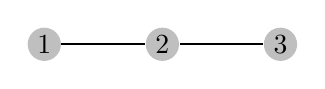
\begin{tikzpicture}[scale=1.5]
    % Draw a 7,11 network
    % First we draw the vertices
    \foreach \pos/\name in {{(1,0)/1}, {(2,0)/2}, {(3,0)/3}}
        \node[vertex] (\name) at \pos {$\name$};
    % Connect vertices with edges 
    \foreach \source/ \dest in {1/2, 2/3}
        \path[edge] (\source) -- (\dest) ;
        
\end{tikzpicture}
\end{center}

If $\pi(Rebel,Rebel,Rebel)>0$, we can construct such equilibrium

\begin{itemize}
\item After nature moves, Rebel 2 chooses $\textbf{revolt}$ if he observes $\theta=(Rebel,Rebel,Rebel)$, and plays \textbf{revolt} in this period. Otherwise, he chooses \textbf{stay} and keeps playing \textbf{stay} afterwards. 
\item After nature moves, Rebel 1 and Rebel 3 play \textbf{stay}.
\item If Rebel 2 chooses \textbf{revolt} in the last period, then Rebel 1 (or Rebel 3) plays \textbf{revolt} in this period; if Rebel 2 chooses \textbf{stay} in the last period, then Rebel 1 (or Rebel 3) keeps playing \textbf{stay} afterwards. 
\end{itemize}

  
}


\subsection{Literature Review}
\frame{
  \frametitle{Related Literature}

  \begin{itemize}
  \item Public good provision.
  \begin{itemize}
  \item One strand: costly information generation. [Lohmann, 1993,1994], [Bolton and Harris, 1999], [Bramoull\'{e}́ and Kranton, 2007]
  \item \underline{Here, add network-monitoring}
  \end{itemize}
  \item Social learning.
  \begin{itemize}
  \item One strand: learning in network. [Goyal, 2012], [Acemoglu et al., 2011], [Chatterjee and Dutta, 2011].
  \item \underline{Here, farsighted-learning in the game}
  \end{itemize}
  \item Repeated game.
  \begin{itemize}
  \item One strand: repeated game in network. [Laclau, 2012], [Wolitzky, 2013], [Wolitzky, 2014]
  \item \underline{Here, incomplete information imperfect monitoring }
  \item One strand: folk theorem with incomplete information imperfect monitoring. [Fudenberg and Yamamoto, 2010] [Fudenberg and Yamamoto, 2011] [Wiseman, 2012] 
  \item \underline{Here, not a folk theorem}. No assumptions on public or private signal generated by single-period actions.
  \end{itemize}
  
\end{itemize}

}



\section{Model}
\subsection{Static Game}
\frame{
  \frametitle{Model}

Network
  \begin{itemize}
  \item $n$ players. Let $N=\{1,...,n\}$ be the set of players. 
 
  \item $G_i$ is a subset of $N$, where $i\in G_i$
  \item $G_i$ is $i$'s neighborhood. $\bar{G}_i=G_i \backslash \{i\}$ is $i$'s neighborhood excluding $i$. 
  \item $G=\{G_i\}_i$ is the network.
 \item $G$ is fixed if $G$ is not random; finite if $N$ is finite; undirected if $j\in G_i\Rightarrow i\in G_j$.
 \begin{definition}
 \begin{enumerate}
 \item A \textit{path} from $i$ to $j$, $i\neq j$ in an undirected network $G$ is a finite sequence $l_1,...,l_q$ such that $l_1=i, l_2\in \bar{G}_{l_1}, l_3\in \bar{G}_{l_2},...,l_q=j$ and $l_1,...,l_q$ are all distinct.
 \item \textit{connectedness}:  An undirected network is connected if and only if for all $i,j$, $i\neq j$ there is a path from $i$ to $j$. 
 \end{enumerate}

\end{definition}
 
  \end{itemize}


}

\frame{
  \frametitle{Model}

Static $k$-threshold game [Chwe 2000]
  \begin{itemize}
 \item Each player $i$'s type $\theta_i\in \Theta_i=\{Rebel,Inert\}$
  \item Denote $\Theta=\times_{i\in N}\Theta_i$
  \item Prior $\pi$ over $\Theta$.
  \item $A_{Rebel_i}=\{\textbf{revolt},\textbf{stay}\}$; $A_{Inert_i}=\{\textbf{inert}\}$
    \item A parameter $k$ with $1\leq k \leq n$
  \item Static game payoff for player $i$: $u_{\theta_i}(a_{\theta_i},a_{-\theta_i})$

  \begin{table}[h]
\begin{tabular}{llll}
$u_{Rebel_i}(a_{Rebel_i},a_{-\theta_i})$ & $=$ & 1 & if $a_{Rebel_i}=\textbf{revolt}$ and $\#\{j:a_{\theta_j}=\textbf{revolt}\}\geq k$ \\
$u_{Rebel_i}(a_{Rebel_i},a_{-\theta_i})$ & $=$ & -1 & if $a_{Rebel_i}=\textbf{revolt}$ and $\#\{j:a_{\theta_j}=\textbf{revolt}\}< k$ \\
$u_{Rebel_i}(a_{Rebel_i},a_{-\theta_i})$ & $=$ & 0 & if $a_{Rebel_i}=\textbf{stay}$ \\
$u_{Inert_i}(a_{Inert_i},a_{-\theta_i})$ & $=$  & 1 &  if  $a_{Inert_i}=\textbf{inert}$
\end{tabular}
\end{table}

  \item Players only know their neighbor's types.
  \end{itemize}


}

\frame{
  \frametitle{Model}

  \begin{itemize}
  \item Denote $[Rebels](\theta)=\{j:\theta_j=Rebel\}$ for $\theta\in \Theta$.
  \item Denote $\# A$ as the cardinality of a finite set $A$.
  \end{itemize} 

}




\subsection{Repeated Game}
\begin{frame}
  \frametitle{Model}
Repeated $k$-threshold game
  \begin{itemize}

  \item Common $\delta$. Time is infinite, discrete.
  \item Nature choose $\theta$ at $0$ period; players play the static $k$-threshold game infinitely repeatedly.
     \item Players perfectly only observe his neighbors' actions. 
    \item $h^{m}_{G_i}$: the history $i$ can observe up to period $m$
   \item $\beta_i(\theta|h^{m}_{G_i})$: $i$'s belief for $\theta$ at period $m$. 
  \item Payoff is hidden.
    \item Equilibrium concept: (weak) sequential Equilibrium.


  \end{itemize}

\end{frame}



\begin{frame}
  \frametitle{Model}

\begin{assumption}
$G$ is commonly known
\end{assumption}

\begin{definition}
$\pi$ has full support if and only if $\pi(\theta)>0$ for all $\theta\in \Theta$.
\end{definition}
\begin{definition}\label{Def_expost_efficient}
A sequential equilibrium is \textit{approaching efficient} (APEX) if and only if for all $\theta$ there is a finite time $T^{\theta}$ such that the tails of actions after $T^{\theta}$ in equilibrium path repeats the ex-post efficient outcome.
\end{definition}
 


\end{frame}




\frame{
  \frametitle{Equilibrium: $k=n$}

\begin{theorem}
\label{prop:not_crowded}
\textbf{In} any fixed, finite, connected, commonly known, undirected (FFCCU) network, \textbf{if} the prior has full support , \textbf{then} for $n$-person repeated $k$-Threshold game with parameter $k=n$ played in such networks, \textbf{there is} a $\delta$ such that a sequential equilibrium which is APEX \textbf{exists}.
\end{theorem}

Proof:
  \begin{itemize}
  \item If there is an Inert neighbor, then play \textbf{stay} forever.
  \item If there is no Inert neighbor, then play \textbf{revolt} until he observe some neighbors play \textbf{stay}, and then play \textbf{stay} forever.
  \item If he deviates, then play \textbf{revolt} forever.
  \item Since networks are FFCCU, there is a finite time $T^{\theta}$ such that ex-post efficient outcome repeats afterwards.

  \end{itemize} 

}

\frame{
  \frametitle{Equilibrium: $k=n$}

$k=n$ is a trivial case.
\begin{itemize}
\item Rebels will never play \textbf{revolt} if one of his neighbor is Inert.
\item $\{\textbf{revolt}, \textbf{stay}\}$ reveals ``no Inert'', ``some Inert''.
\item When someone deviates, group punishment is not needed. 
\end{itemize}

}

\frame{
  \frametitle{Equilibrium: $k<n$}

$k<n$ is not a trivial case
\begin{itemize}
\item Rebels \textbf{may} play \textbf{revolt} if one of his neighbor is Inert.
\item $\{\textbf{revolt}, \textbf{stay}\}$ has to reveal more information.
\item When someone deviates, group punishment may be needed. 
\end{itemize}

}

\begin{frame}
  \frametitle{Equilibrium: $k<n$}

\underline{Rebels \textbf{may} play \textbf{revolt} even if one of his neighbor is Inert}. 
\begin{itemize}
\item Let $k=2$
\item Assume $\theta=(Rebel_1,Inert_2,Rebel_3)$.
\item Let $G$ be
\begin{center}
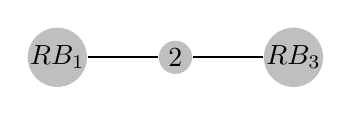
\begin{tikzpicture}[scale=1.5]
    % Draw a 7,11 network
    % First we draw the vertices
    \foreach \pos/\name in {{(1,0)/RB_1}, {(2,0)/2}, {(3,0)/RB_3}}
        \node[vertex] (\name) at \pos {$\name$};
    % Connect vertices with edges 
    \foreach \source/ \dest in {RB_1/2, 2/RB_3}
        \path[edge] (\source) -- (\dest) ;
        
\end{tikzpicture}
\end{center}
\end{itemize}
 
\begin{enumerate}

\item Inert 2 block the information transmission.
\item This is an incomplete information game without communication

\item Rebel 1 still has incentive to play \textbf{revolt}. 
\begin{itemize}
\item $\pi(\{\theta:\theta_3=Rebel\})$ is high
\item Rebel 3 will play revolt.
\end{itemize}
\item Generally, achieving APEX is impossible.
\end{enumerate}



\end{frame}

\begin{frame}
  \frametitle{Equilibrium: $k<n$}

Given $G$,
\begin{definition}
\textbf{Strong connectedness} $\Leftrightarrow$ for every pair of Rebels, there is a path consisting of Rebels to connect them.
\end{definition}  

\begin{definition}
\textbf{Full support on strong connectedness}$\Leftrightarrow$ 
\begin{enumerate}
\item $1>\pi(\theta)>0$ whenever $\theta$ has strong connectedness.
\item $\pi(\theta)=0$ whenever $\theta$ did not satisfy strong connectedness.
\end{enumerate}

\end{definition}  

\end{frame}



\begin{frame}
  \frametitle{Equilibrium: $k<n$}

\underline{$\{\textbf{revolt}, \textbf{stay}\}$ has to reveal more information}. Suppose Rebel 3, 5 ``talk to'' Rebel 1, 2. 
  \begin{itemize}
  \item Let $k=5$
\begin{center} 
  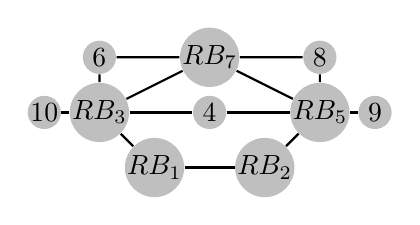
\begin{tikzpicture}[scale=0.7]
    % First we draw the vertices
    \foreach \pos/\name in {{(2,1)/RB_1}, {(4,1)/RB_2}, {(1,2)/RB_3}, {(5,2)/RB_5}, {(3,3)/RB_7}, {(3,2)/4}, {(1,3)/6}, {(5,3)/8}, {(6,2)/9}, {(0,2)/10}}
        \node[vertex] (\name) at \pos {$\name$};
        
%        \foreach \pos/\name in {{(3,2)/4_L}, {(1,3)/6_L}, {(5,3)/8_L}, {(6,2)/9_L}, {(0,2)/10_L}}
%   \node[selected vertex] (\name) at \pos {$\name$};
    
    % Connect vertices with edges 
    \foreach \source/ \dest in {RB_1/RB_2, RB_1/RB_3, RB_2/RB_5, RB_3/4, RB_3/6, RB_3/RB_7, 4/RB_5, RB_5/RB_7, RB_5/8, RB_5/9,6/RB_7, RB_7/8, RB_3/10}
        \path[edge] (\source) -- (\dest) ;
\end{tikzpicture}
\end{center} 
\end{itemize}

\begin{itemize}
\item Let $k=6$ 
\begin{center} 
  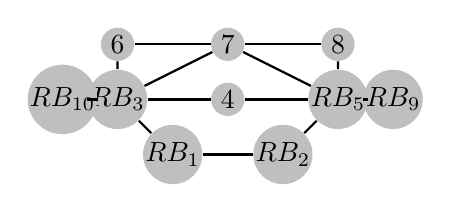
\begin{tikzpicture}[scale=0.7]
    % First we draw the vertices
    \foreach \pos/\name in {{(2,1)/RB_1}, {(4,1)/RB_2}, {(1,2)/RB_3}, {(5,2)/RB_5}, {(3,3)/7}, {(3,2)/4}, {(1,3)/6}, {(5,3)/8}, {(6,2)/RB_9}, {(0,2)/RB_{10}}}
        \node[vertex] (\name) at \pos {$\name$};
        
%        \foreach \pos/\name in {{(3,2)/4_L}, {(1,3)/6_L}, {(5,3)/8_L}, {(6,2)/9_L}, {(0,2)/10_L}}
%   \node[selected vertex] (\name) at \pos {$\name$};
    
    % Connect vertices with edges 
    \foreach \source/ \dest in {RB_1/RB_2, RB_1/RB_3, RB_2/RB_5, RB_3/4, RB_3/6, RB_3/7, 4/RB_5, RB_5/7, RB_5/8, RB_5/RB_9,6/7, 7/8, RB_3/RB_{10}}
        \path[edge] (\source) -- (\dest) ;
\end{tikzpicture}
\end{center} 
\end{itemize}

\begin{itemize}
\item ``Talking about how many nearby Rebels'' is not enough.
\item  ``Talking about how many nearby Rebels''  and ``Talking about nearby Rebels' locations'' 
\end{itemize}



\end{frame}


\begin{frame}
  \frametitle{Equilibrium: $k<n$}

\underline{When someone deviates, group punishment may be needed}.

\begin{itemize}
\item Let $k=4$
\begin{center}
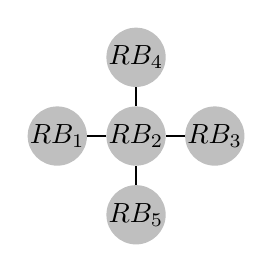
\begin{tikzpicture}[scale=1]
    % Draw a 7,11 network
    % First we draw the vertices
    \foreach \pos/\name in {{(1,1)/RB_1}, {(2,1)/RB_2}, {(3,1)/RB_3}, {(2,2)/RB_4}, {(2,0)/RB_5}}
        \node[vertex] (\name) at \pos {$\name$};
    % Connect vertices with edges 
    \foreach \source/ \dest in {RB_1/RB_2, RB_2/RB_3, RB_4/RB_2, RB_2/RB_5}
        \path[edge] (\source) -- (\dest) ;
        
\end{tikzpicture}
\end{center}
\end{itemize}

\begin{enumerate}
\item Rebel 1 can only be monitored by Rebel 2.
\item Given some strategies, suppose Rebel 2,3,4,5 can coordinate at period $T$ and play \textbf{revolt} forever.
\item If Rebel 1 deviate at period $T-1$, Rebel 2 has no incentive to punish him.
\begin{itemize}
\item Different from the case $k=n=5$
\end{itemize}
\end{enumerate}
\end{frame}






\begin{frame}
  \frametitle{Equilibrium: $k<n$}



\begin{theorem}
\label{thm_main_result}
\textbf{In any} FFCCU network without cycles, \textbf{if} $\theta$ has strong connectedness and $\pi$ has full support on strong connectedness, \textbf{then} for $n$-person repeated $k$-Threshold game with parameter $1\leq k < n$ played in networks, \textbf{there is} a $\delta$ such that a weak sequential equilibrium which is APEX \textbf{exists}.
\end{theorem}

\begin{definition}\textbf{Cycles:}
A FFCCU network is without cycles $\Leftrightarrow$ the path from $i$ to $j$, for $i\neq j$, is unique. 
\end{definition}

\end{frame}







\section{Equilibrium construction}
\subsection{Equilibrium construction}

\begin{frame}
  \frametitle{Equilibrium construction}

\underline{$\{\textbf{revolt}, \textbf{stay}\}$ has to reveal more information}
\begin{itemize}
\item Indexing each node $i$ as a distinct prime number $x_i$.
\item Rebel 3 report $x_1\times x_7 \times x_1$ to Rebel 1 by sending a finite sequence 
\[\textbf{stay},...,\textbf{stay},\underbrace{\textbf{revolt},\textbf{stay},...,\textbf{stay}}_{x_1\times x_7 \times x_3}\]
\end{itemize}
\begin{center} 
  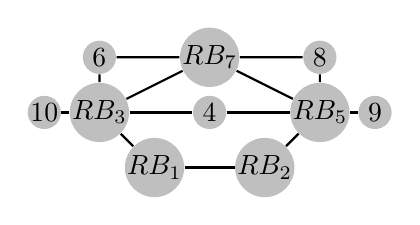
\begin{tikzpicture}[scale=0.7]
    % First we draw the vertices
    \foreach \pos/\name in {{(2,1)/RB_1}, {(4,1)/RB_2}, {(1,2)/RB_3}, {(5,2)/RB_5}, {(3,3)/RB_7}, {(3,2)/4}, {(1,3)/6}, {(5,3)/8}, {(6,2)/9}, {(0,2)/10}}
        \node[vertex] (\name) at \pos {$\name$};
        
%        \foreach \pos/\name in {{(3,2)/4_L}, {(1,3)/6_L}, {(5,3)/8_L}, {(6,2)/9_L}, {(0,2)/10_L}}
%   \node[selected vertex] (\name) at \pos {$\name$};
    
    % Connect vertices with edges 
    \foreach \source/ \dest in {RB_1/RB_2, RB_1/RB_3, RB_2/RB_5, RB_3/4, RB_3/6, RB_3/RB_7, 4/RB_5, RB_5/RB_7, RB_5/8, RB_5/9,6/RB_7, RB_7/8, RB_3/10}
        \path[edge] (\source) -- (\dest) ;
\end{tikzpicture}
\end{center} 

\begin{center} 
  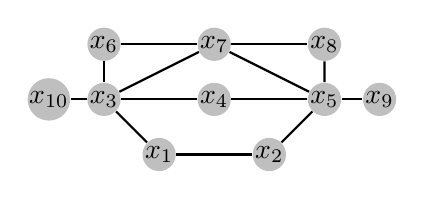
\begin{tikzpicture}[scale=0.7]
    % First we draw the vertices
    \foreach \pos/\name in {{(2,1)/x_1}, {(4,1)/x_2}, {(1,2)/x_3}, {(5,2)/x_5}, {(3,3)/x_7}, {(3,2)/x_4}, {(1,3)/x_6}, {(5,3)/x_8}, {(6,2)/x_9}, {(0,2)/x_{10}}}
        \node[vertex] (\name) at \pos {$\name$};
        
%        \foreach \pos/\name in {{(3,2)/4_L}, {(1,3)/6_L}, {(5,3)/8_L}, {(6,2)/9_L}, {(0,2)/10_L}}
%   \node[selected vertex] (\name) at \pos {$\name$};
    
    % Connect vertices with edges 
    \foreach \source/ \dest in {x_1/x_2, x_1/x_3, x_2/x_5, x_3/x_4, x_3/x_6, x_3/x_7, x_4/x_5, x_5/x_7, x_5/x_8, x_5/x_9,x_6/x_7, x_7/x_8, x_3/x_{10}}
        \path[edge] (\source) -- (\dest) ;
\end{tikzpicture}
\end{center} 

\end{frame}


\begin{frame}
  \frametitle{Equilibrium construction}

Using $\{\textbf{revolt}, \textbf{stay}\}$-sequences to transmit information
\begin{itemize}
\item  Naively, we may let Rebel 3 report $\rightarrow$ Rebel 5 report $\rightarrow$ Rebel 1 report $\rightarrow$...


\begin{center} 
  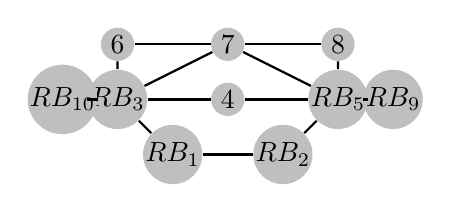
\begin{tikzpicture}[scale=0.7]
    % First we draw the vertices
    \foreach \pos/\name in {{(2,1)/RB_1}, {(4,1)/RB_2}, {(1,2)/RB_3}, {(5,2)/RB_5}, {(3,3)/7}, {(3,2)/4}, {(1,3)/6}, {(5,3)/8}, {(6,2)/RB_9}, {(0,2)/RB_{10}}}
        \node[vertex] (\name) at \pos {$\name$};
        
%        \foreach \pos/\name in {{(3,2)/4_L}, {(1,3)/6_L}, {(5,3)/8_L}, {(6,2)/9_L}, {(0,2)/10_L}}
%   \node[selected vertex] (\name) at \pos {$\name$};
    
    % Connect vertices with edges 
    \foreach \source/ \dest in {RB_1/RB_2, RB_1/RB_3, RB_2/RB_5, RB_3/4, RB_3/6, RB_3/7, 4/RB_5, RB_5/7, RB_5/8, RB_5/RB_9,6/7, 7/8, RB_3/RB_{10}}
        \path[edge] (\source) -- (\dest) ;
\end{tikzpicture}
\end{center} 
\item $\rightarrow$ since network is finite, then some Rebels will know the true state $\rightarrow$ some more Rebels will know the true state. $\rightarrow$...$\rightarrow$ all Rebels will know the true state $\rightarrow$...$\rightarrow$ all Rebels will know all Rebels ... know the true state, etc.
\item APEX requires that there is a timing to play \textbf{revolt} or \textbf{stay} forever.
\begin{enumerate}
\item However, calculating such timing given all possible $\theta$ is tedious.
\item Higher-order belief is apparently a giant object.
\end{enumerate} 
\end{itemize}

\end{frame}


\begin{frame}
  \frametitle{Equilibrium construction}

Using $\{\textbf{revolt}, \textbf{stay}\}$-sequences to transmit information 
\begin{enumerate}
\item about $\theta$ (\textbf{Reporting messages})
\item about ``Have some Rebels known $\#[Rebels](\theta)\geq k$ or $\#[Rebels](\theta)< k$?'' (\textbf{Coordination messages} )
\begin{itemize}
\item To bypass the tracking of higher-order belief when network is finite.
\end{itemize}
\end{enumerate}
Specifically,
\[\underbrace{\langle\text{coordination period}\rangle}_{0-block}\underbrace{\langle\text{reporting period}\rangle \langle\text{coordination period}\rangle}_{1-block}...\]

\begin{itemize}
\item If some Rebels know the relevant information, then send coordination messages to other Rebels.
\item And then Rebels play \textbf{revolt} or \textbf{stay} after coordination period. 
\end{itemize}

\end{frame}


\begin{frame}
  \frametitle{Equilibrium construction}

\underline{When someone deviates, group punishment may be needed}.
 
  \begin{itemize}
  \item Recall
    \begin{center}
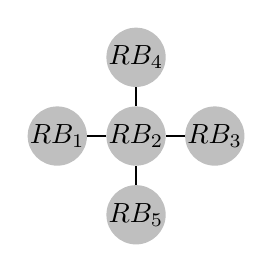
\begin{tikzpicture}[scale=1]
    % Draw a 7,11 network
    % First we draw the vertices
    \foreach \pos/\name in {{(1,1)/RB_1}, {(2,1)/RB_2}, {(3,1)/RB_3}, {(2,2)/RB_4}, {(2,0)/RB_5}}
        \node[vertex] (\name) at \pos {$\name$};
    % Connect vertices with edges 
    \foreach \source/ \dest in {RB_1/RB_2, RB_2/RB_3, RB_4/RB_2, RB_2/RB_5}
        \path[edge] (\source) -- (\dest) ;
        
\end{tikzpicture}
\end{center}
   \item Rebel 1 has less incentive to send information.
   \item Rebel 2 have strictly more information than all of his neighbors.
   
  \item Characterize those Rebels who have strictly more information about $\theta$ than any of their neighbors - \textbf{Information hierarchy}.

  \end{itemize}

\end{frame}


\begin{frame}
  \frametitle{Equilibrium construction}

\[\underbrace{\langle\text{coordination period}\rangle}_{0-block}\underbrace{\langle\text{reporting period}\rangle \langle\text{coordination period}\rangle}_{1-block}...\]
\begin{enumerate}
\item Step 1: Characterize information hierarchy for each $t$-block.
\item Step 2: Build reporting and coordination messages in the path, and show the in-path belief updating.
\item Step 3: Set up off-path belief.
\end{enumerate}

\end{frame}





\subsection{Information Hierarchy}

\begin{frame}
  \frametitle{Information Hierarchy}

At $0$-block, let
  \begin{itemize}
  \item \[R^0=[Rebels](\theta)\]
  \end{itemize}


\end{frame}



\begin{frame}
  \frametitle{Information Hierarchy}

At $1$-block, let
\begin{eqnarray*}
N^0_i & \equiv &  G_i\\
I^0_i & \equiv & G_i\cap R^0\\
\end{eqnarray*}

Define $\leq^0$ by
\[i\in \leq^0 \Leftrightarrow \exists  j\in \bar{G}_i (I^0_i\subseteq N^0_j\cap R^0)\] 
\begin{itemize}
\item $\leq^0$ is the set of players whose Rebel neighbors are covered by his neighbors' Rebel neighbors.
\end{itemize}

Let 
\begin{eqnarray*}
R^{1} \equiv \{i\in R^0|i\notin \leq^0\}
\end{eqnarray*}

\begin{itemize}
\item $R^1$ are those Rebels whose Rebel neighbors can not covered by all of his neighbors' Rebel neighbors.
\end{itemize}


\end{frame}

\begin{frame}
  \frametitle{Information Hierarchy}

Ex., Rebel 1 is a non-$R^1$ node. Rebel 2 is a $R^1$ node. 

 \begin{center}
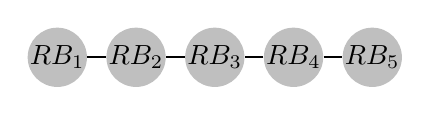
\begin{tikzpicture}[scale=1]
    % Draw a 7,11 network
    % First we draw the vertices
    \foreach \pos/\name in {{(1,1)/RB_1}, {(2,1)/RB_2}, {(3,1)/RB_3}, {(4,1)/RB_4}, {(5,1)/RB_5}}
        \node[vertex] (\name) at \pos {$\name$};
    % Connect vertices with edges 
    \foreach \source/ \dest in {RB_1/RB_2, RB_2/RB_3, RB_4/RB_3, RB_4/RB_5}
        \path[edge] (\source) -- (\dest) ;
        
\end{tikzpicture}
\end{center}
\end{frame}


\begin{frame}
  \frametitle{Information Hierarchy}

In $t+1$-block, denote
\begin{eqnarray*}
N^t_i & \equiv & \bigcup_{k\in I^{t-1}_i}G_k \\
I^t_i & \equiv & \bigcup_{k\in G_i\cap R^t}I^{t-1}_k
\end{eqnarray*}
\begin{itemize}
\item $N^t_i$ is $i$'s \textit{extended} neighborhood given $i$'s information $I^{t-1}_i$
\item $I^t_i$ is $i$'s \textit{extended} Rebel neighbors given $j$'s information $I^{t-1}_j$, where $j$ is a $R^{t}$ Rebel. 
\end{itemize}


Define $\leq^t$ by
\[i\in \leq^t \Leftrightarrow \exists j\in \bar{G}_i(I^t_i\subseteq N^t_j\cap R^0)\] 
\begin{itemize}
\item $\leq^t$ is the set of players whose extended Rebel neighbors are covered by his neighbors' extended Rebel neighbors.
\end{itemize}

Let 
\begin{eqnarray*}
R^{t+1} \equiv  \{i\in R^t|i\notin \leq^t\}
\end{eqnarray*}


\end{frame}

\begin{frame}
  \frametitle{Information Hierarchy}

\begin{enumerate}
\item Rebel 1 is a non-$R^1$ node. Rebel 2 is a $R^1$ node. Rebel 3 is a $R^1$ node.
\item Rebel 1 is a non-$R^2$ node. Rebel 2 is a non-$R^2$ node. Rebel 3 is a $R^2$ node.
\end{enumerate}


 \begin{center}
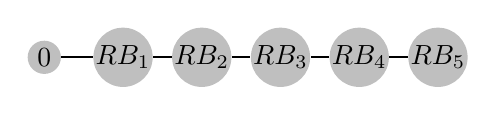
\begin{tikzpicture}[scale=1]
    % Draw a 7,11 network
    % First we draw the vertices
    \foreach \pos/\name in {{(0,1)/0}, {(1,1)/RB_1}, {(2,1)/RB_2}, {(3,1)/RB_3}, {(4,1)/RB_4}, {(5,1)/RB_5}}
        \node[vertex] (\name) at \pos {$\name$};
    % Connect vertices with edges 
    \foreach \source/ \dest in {0/RB_1,RB_1/RB_2, RB_2/RB_3, RB_4/RB_3, RB_4/RB_5}
        \path[edge] (\source) -- (\dest) ;
        
\end{tikzpicture}
\end{center}

\begin{theorem}
\label{lemma_empty}
If the network is FFCCU without cycle and if the state has strong connectedness, then 
\[R^0\neq \emptyset \Rightarrow \exists t\geq 0(\exists i\in R^t(I^t_i=R^0))\]
\end{theorem} 
\end{frame}










\section{Equilibrium path}
\begin{frame}
\frametitle{Equilibrium path}

At $t$-block, 
\begin{itemize}
\item $RP^t$: the reporting period
\item $CD^t$: the coordination period
\begin{itemize}
\item There are some sub-periods in divisions in a coordination period.
\[\overbrace{\langle\underbrace{\langle \cdot \rangle \cdot \cdot \cdot \langle \cdot \rangle}_{\text{sub-blocks}}\rangle \langle\underbrace{\langle \cdot \rangle \cdot \cdot \cdot \langle \cdot \rangle}_{\text{sub-blocks}} \rangle \langle\underbrace{\langle \cdot \rangle \cdot \cdot \cdot \langle \cdot \rangle}_{\text{sub-blocks}}\rangle}^{\text{coordination period}}\] 
\item $CD^t_{p,q}$: the $p$ sub-blocks in $q$ division in $t$-block coordination period.
\end{itemize}
\item $\langle RP^t \rangle$: the reporting messages
\item $\langle CD^t \rangle$: the coordination messages
\item Players use messages, which length is the same as the length of corresponding period.   

\end{itemize}



\end{frame}


\begin{frame}
\frametitle{Equilibrium path}

At $t$-block ($t>0$), denote
\begin{itemize}
\item $\langle I^{t-1}_i\rangle$=$\textbf{s},...,\textbf{s},\underbrace{\textbf{r},\textbf{s},...,\textbf{s}}_{\times_{j\in I^{t-1}_i}x_j}$
\item $\langle \textbf{stay} \rangle$=$\textbf{s},...,\textbf{s}$
\end{itemize}

At $t$-block ($t>0$), ideally,
\begin{itemize}
\item Let $R^t$ report $\langle I^{t-1} \rangle$ truthfully in reporting period.
\item Let $R^t$ send ``coordination messages'' to coordinate in coordination period.
\item Let non-$R^t$ report $\langle \textbf{stay} \rangle$ truthfully in reporting period.
\end{itemize}


Not so obvious. Sending message incurs expected cost and therefore players may want to deviate from truthful reporting.


\end{frame}


\begin{frame}
\frametitle{Equilibrium path}

A free rider problem. Pivotal player case 1.

\begin{itemize}
\item $k=5$
\item Assume players' strategies are starting with a $RP$ and then a $CD$ follows. 
\item Assume there is a action-irrelevant message $\langle M \rangle$.
\item When Rebel observe $\langle M \rangle$ immediately after $PR$, they play \textbf{revolt} forever; Otherwise, play \textbf{stay} forever.

\end{itemize}

\begin{center}
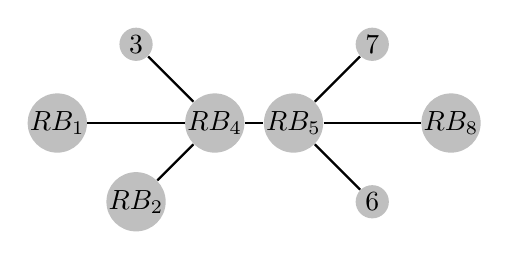
\begin{tikzpicture}[scale=1]
    % Draw a 7,11 network
    % First we draw the vertices
    \foreach \pos/\name in {{(1,2)/RB_1}, {(2,1)/RB_2}, {(2,3)/3}, {(3,2)/RB_4}, {(4,2)/RB_5}, {(5,1)/6}, {(5,3)/7}, {(6,2)/RB_8}}
        \node[vertex] (\name) at \pos {$\name$};
    
    
    % Connect vertices with edges 
    \foreach \source/ \dest in {RB_1/RB_4, RB_2/RB_4,3/RB_4,RB_4/RB_5, RB_5/6, RB_5/7, RB_5/RB_8}
        \path[edge] (\source) -- (\dest) ;
        
\end{tikzpicture}
\end{center}

\begin{itemize}
\item \textbf{Problem}: Both Rebel 4 and Rebel 5 are pivotal; they will shift to play $\langle \textbf{stay} \rangle$ if others report truthfully.
\end{itemize}


\end{frame}


\begin{frame}
\frametitle{Equilibrium path}

Pivotal Player Case 2

\begin{itemize}
\item $k=6$
\item Assume players' strategies are starting with a $RP$ and then a $CD$ follows. 
\item Assume there is a action-irrelevant message $\langle M \rangle$.
\item When Rebel observe $\langle M \rangle$ immediately after $PR$, they play \textbf{revolt} forever; Otherwise, play \textbf{stay} forever.

\end{itemize}

\begin{center}
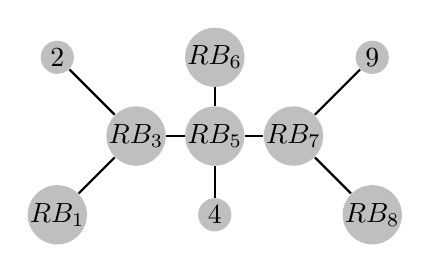
\begin{tikzpicture}[scale=1]
    % Draw a 7,11 network
    % First we draw the vertices
    \foreach \pos/\name in {{(1,1)/RB_1}, {(1,3)/2}, {(2,2)/RB_3}, {(3,1)/4}, {(3,2)/RB_5}, {(3,3)/RB_6}, {(4,2)/RB_7}, {(5,1)/RB_8}, {(5,3)/9}}
        \node[vertex] (\name) at \pos {$\name$};
    
    
    % Connect vertices with edges 
    \foreach \source/ \dest in {RB_1/RB_3, 2/RB_3,RB_3/RB_5,4/RB_5, RB_6/RB_5, RB_5/RB_7, RB_7/RB_8, RB_7/9}
        \path[edge] (\source) -- (\dest) ;
        
\end{tikzpicture}
\end{center}

\begin{itemize}
\item \textbf{Problem}: Rebel 5 is pivotal; he shifts to play $\langle \textbf{stay} \rangle$. Why?
\end{itemize}

\end{frame}

\begin{frame}
\frametitle{Equilibrium path}

Pivotal Player Case 3

\begin{itemize}
\item $k=6$
\item Assume players' strategies are starting with a $RP$ and then a $CD$ follows. 
\item Assume there is a action-irrelevant message $\langle M \rangle$.
\item When Rebel observe $\langle M \rangle$ immediately after $PR$, they play \textbf{revolt} forever; Otherwise, play \textbf{stay} forever.

\end{itemize}

\begin{center}
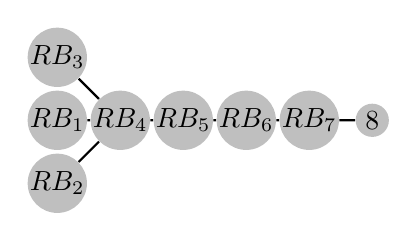
\begin{tikzpicture}[scale=0.8]
    % Draw a 7,11 network
    % First we draw the vertices
    \foreach \pos/\name in {{(2,2)/RB_1}, {(2,1)/RB_2}, {(2,3)/RB_3}, {(3,2)/RB_4}, {(4,2)/RB_5}, {(5,2)/RB_6}, {(6,2)/RB_7}, {(7,2)/8}}
        \node[vertex] (\name) at \pos {$\name$};
    
    
    % Connect vertices with edges 
    \foreach \source/ \dest in {RB_1/RB_4, RB_2/RB_4,RB_3/RB_4,RB_4/RB_5, RB_5/RB_6, RB_6/RB_7, RB_7/8}
        \path[edge] (\source) -- (\dest) ;
        
\end{tikzpicture}
\end{center}

\begin{itemize}
\item \textbf{Problem}: Rebel 4 is pivotal; he shifts to play $\langle \textbf{stay} \rangle$. Why?
\end{itemize}

\end{frame}


\begin{frame}
\frametitle{Equilibrium path}

\begin{itemize}
\item Thus, some Rebels have incentives to deviate from truthfully reporting $\langle I^{t-1} \rangle$ to $\langle \textbf{stay} \rangle$.
\begin{itemize}
\item Free rider problems occurs.
\item The ``meaning'' of $\langle \textbf{stay} \rangle$ is vague.
\end{itemize}
\item Remedy: Create another message, $\langle 1 \rangle= \textbf{s},...,\textbf{s},\textbf{r}$, as the message used by pivotal player.
\item Remedy: If there is a free rider problem, choose some players as free rider and choose some to contribute. 
\item Remedy: Let Rebels' continuation behavior be not only contingent on coordination message $M$ but also on reporting message.

\item Good news: The pivotal problems can be identified as the above three cases.
\item Good news: The free rider problem can be identified as the above case.
\begin{itemize}
\item Two nearby Rebels.
\end{itemize}

\end{itemize}

\end{frame}





\begin{frame}
\frametitle{Equilibrium path}

\begin{itemize}
\item Good news: With suitable coordination messages and continuation behavior
\begin{enumerate}
\item Pivotal players will not deviate from playing $\langle 1 \rangle$.
\item Only pivotal players will play $\langle 1 \rangle$
\end{enumerate}
\item Good news: the belief updating after $CD^t$, $t>0$ in the equilibrium path will be

\end{itemize}


\begin{table}[ht]
\caption{Belief updating after $CD^t_{1,2}$, $t>0$}
\label{Table_blf_up_cdt12}
\begin{center}
\begin{tabular}{l c c c}
In $RP^t$ 	 	&  	In $CD^t_{1,1}$		&  In $CD^t_{1,2}$	  &\\
\hline
\hline
$i$ plays 		                             &  	$i$ plays		&				$i$ plays			& The events $j$ believe with probability one  \\
\hline
$\langle  \textbf{stay} \rangle$ 	& 	$\langle \mathbf{1}_i \rangle$	&  $\langle \textbf{stay} \rangle$ &  $i\notin R^t$ \\
$\langle  {I^{t-1}_i} \rangle$ 		&  $\langle \textbf{stay} \rangle$	&	$\langle \textbf{stay} \rangle$ &  $\#[Rebels](\theta)< k$   \\
$\langle  {I^{t-1}_i} \rangle$ 		&  $\langle \mathbf{1}_i \rangle$	&	$\langle \textbf{stay} \rangle$ &  $\#[Rebels](\theta)\geq k$    \\
$\langle  {I^{t-1}_i} \rangle$ 		&  $\langle \mathbf{1}_i \rangle$	&	$\langle \mathbf{1}_i \rangle$ &  $i\in R^t$  \\
$\langle 1 \rangle$ 		             &  $\langle \textbf{stay} \rangle$	&	$\langle \textbf{stay} \rangle$ &  $\#[Rebels](\theta)< k$\\
$\langle 1 \rangle$ 		             &  $\langle \mathbf{1}_i \rangle$	&	$\langle \textbf{stay} \rangle$ & $\#[Rebels](\theta)\geq k$
\end{tabular}
\end{center}
\end{table}
, where, $\langle \mathbf{1}_i \rangle=\textbf{s},...,\textbf{s},\underbrace{\textbf{r},\textbf{s},...,\textbf{s}}_{x_i}$
\end{frame}




\begin{frame}
\frametitle{Off-path Belief}

Whenever Rebel $i$ detects a deviation at $s$ period, he forms the belief 
\begin{equation}
\label{eq_grim_trigger}
\sum_{\theta \in \{\theta:\theta_j=Inert,j\notin G_i\}}\beta^{\pi,\tau}_{G_i}({\theta}|h^{s^{'}}_{G_i})=1
\end{equation}
for all $s^{'}\geq s$. 

\begin{enumerate}
\item If $\# I^0_i<k$, he will play \textbf{stay} forever.
\item This off-path belief then serve as a grim trigger.
\end{enumerate}




\end{frame}


\begin{frame}
\frametitle{Off-path Belief}

Without $\langle 1 \rangle$, using this grim-trigger-like belief may not sustain APEX
\begin{itemize}
\item $k=5$

\end{itemize}

\begin{center}

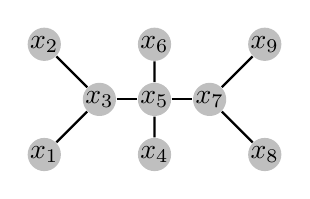
\begin{tikzpicture}[scale=0.7]
    % Draw a 7,11 network
    % First we draw the vertices
    \foreach \pos/\name in {{(1,1)/x_1}, {(1,3)/x_2}, {(2,2)/x_3}, {(3,1)/x_4}, {(3,2)/x_5}, {(3,3)/x_6}, {(4,2)/x_7}, {(5,1)/x_8}, {(5,3)/x_9}}
        \node[vertex] (\name) at \pos {$\name$};
    
    
    % Connect vertices with edges 
    \foreach \source/ \dest in {x_1/x_3, x_2/x_3,x_3/x_5,x_4/x_5, x_6/x_5, x_5/x_7, x_7/x_8, x_7/x_9}
        \path[edge] (\source) -- (\dest) ;
        
\end{tikzpicture}

\end{center}

\begin{center}
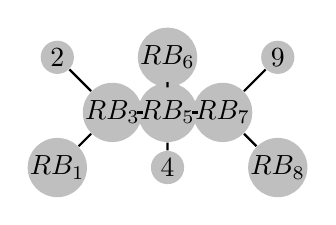
\begin{tikzpicture}[scale=0.7]
    % Draw a 7,11 network
    % First we draw the vertices
    \foreach \pos/\name in {{(1,1)/RB_1}, {(1,3)/2}, {(2,2)/RB_3}, {(3,1)/4}, {(3,2)/RB_5}, {(3,3)/RB_6}, {(4,2)/RB_7}, {(5,1)/RB_8}, {(5,3)/9}}
        \node[vertex] (\name) at \pos {$\name$};
    
    
    % Connect vertices with edges 
    \foreach \source/ \dest in {RB_1/RB_3, 2/RB_3,RB_3/RB_5,4/RB_5, RB_6/RB_5, RB_5/RB_7, RB_7/RB_8, RB_7/9}
        \path[edge] (\source) -- (\dest) ;
        
\end{tikzpicture}
\end{center}

\begin{itemize}
\item \textbf{Problem}: Without $\langle 1 \rangle$ being considered as an in-path strategies; 
\item Rebel 4 is pivotal; He shifts to report $x_3\times x_5 \times x_7$ instead of $x_3\times x_5 \times x_7 \times x_6$. 
\item Coordination can be made, but Rebel 6 is out of coordination since he detects a deviation.
\end{itemize}





\end{frame}

\begin{frame}
\frametitle{Equilibrium: $k<n$: Discussion}

\begin{itemize}
\item From the above steps, an APEX equilibrium is constructed.
\item We can relaxed the assumption that payoff is hidden.
\begin{itemize}
\item payoff is perfectly observed: easy to construct an APEX equilibrium.
\item payoff is noisy: with full support assumption, the existing equilibrium is APEX
\end{itemize}
\item This proof is still open for FFCCU network with cycles.
\item Off-path belief did not satisfy full consistency property for FFCCU network without cycles.
\begin{itemize}
\item Belief updating is had to track
\item Imperfect monitoring impedes the group punishments.
\end{itemize}
\item Prime number indexing also works for other discreet and finite state space.


\end{itemize}


\end{frame}




\begin{frame}

\frametitle{Conclusion}


\begin{enumerate}
\item I show that, without cheap talk, in this repeated $k$-threshold game played in FFCCU networks without cycles, coordination still can happen.
\begin{itemize}
\item Using sequence of actions to communicate.
\end{itemize}
\item The equilibrium is constructive and does not rely on public or private signals other than actions.
\item We can use prime number to index the states given that states are discrete and finite.
\item For the network with circle, it is still remaining to tackle with.
\end{enumerate}
\end{frame}










\end{document}
